
\begin{frame}{Kết luận}
    \textbf{Đóng góp chính:}
    \begin{enumerate}
        \item Đề xuất kiến trúc \textbf{VRAE} tích hợp:
        \begin{itemize}
            \item Kết nối dọc (Vertical Residual)
            \item Khối bổ trợ (Auxiliary Block)
            \item Cơ chế hội tụ đặc trưng đa cấp
        \end{itemize}
        \item Giải quyết bài toán cân bằng:
        \begin{itemize}
            \item Độ chính xác phục hồi (PSNR > 31 dB, SSIM > 0.89)
            \item Chi phí tính toán (194 FPS với VRAE3)
        \end{itemize}
        \item Vượt trội so với các phương pháp hiện có:
        \begin{itemize}
            \item Tăng PSNR ~20\% so với AE cùng độ sâu
            \item Vượt GAN và Flow-based về cả chất lượng và tốc độ
        \end{itemize}
        \item Công bố bài báo tại SOICT 2025
    \end{enumerate}
\end{frame}



% \begin{frame}{Công bố khoa học}
%     \begin{block}{Bài báo được chấp nhận}
%         \textbf{Tên bài báo:} "VRAE: Vertical Residual Autoencoder for License Plate Denoising and Deblurring"
        
%         \vspace{0.2cm}
%         \textbf{Hội nghị:} SOICT 2025 (Hội nghị Quốc tế về Công nghệ Thông tin và Truyền thông lần thứ 14)
        
%         \vspace{0.2cm}
%         \textbf{Tác giả:} Nguyễn Tất Cường (tác giả chính)
        
%         \vspace{0.2cm}
%         \textbf{Năm:} 2025
%     \end{block}
    
%     \begin{figure}
%         \centering
%         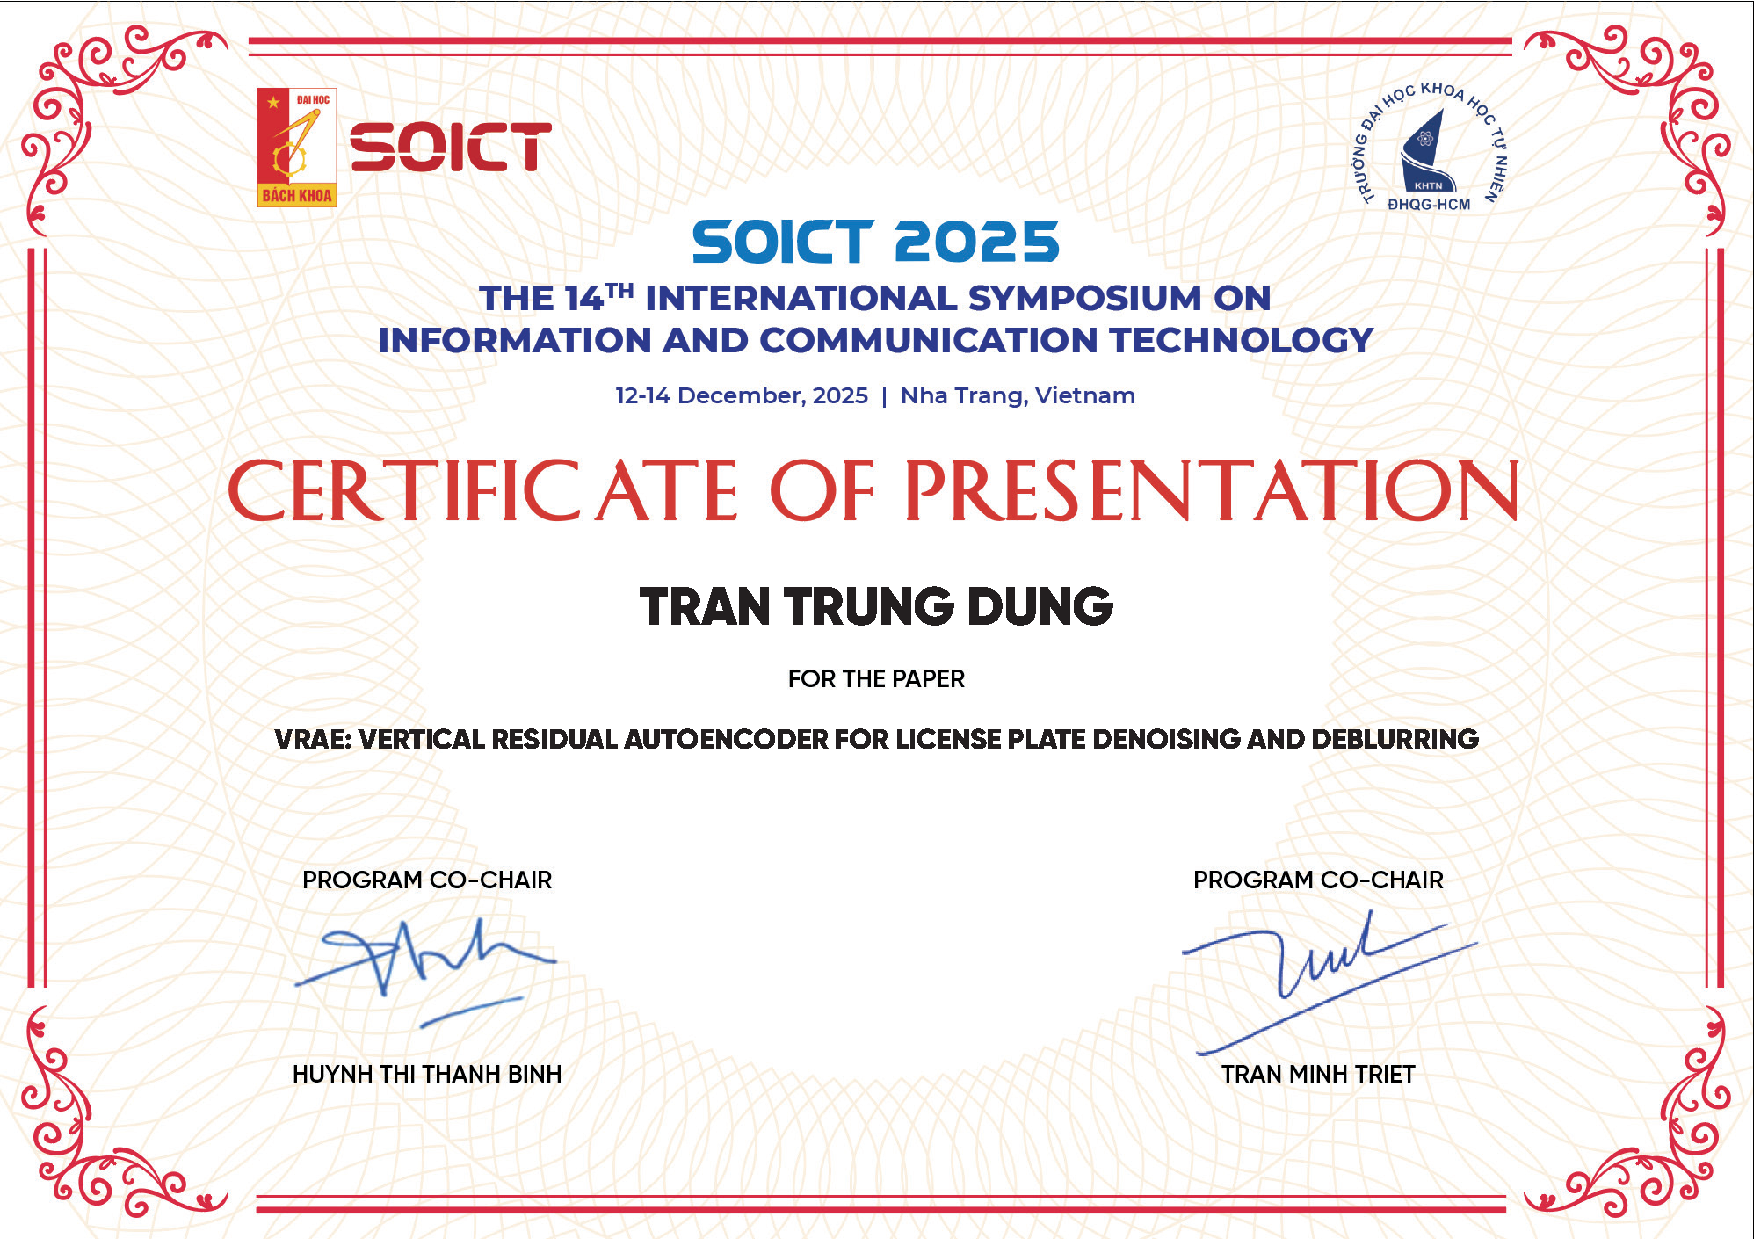
\includegraphics[width=0.5\linewidth]{images/certificate.pdf}
%         \caption{Minh chứng bài báo được trình bày tại SOICT 2025}
%     \end{figure}
% \end{frame}


